\chapter{Results}
In this section the results from the FLEXPART and FLEXDUST model simulations are presented following the methods described in the previous sections. First the results from the model sensitivity experiments are shown \Cref{sec:sensitvity_experiment} and then the model evaluation in \Cref{sec:model_eval}

\section{Model sensitivity experiments}\label{sec:sensitvity_experiment}
\subsection{Sensitivity to forcing data}

\begin{figure}[htpb]
    \centering
    \includegraphics[width=\textwidth]{texfiles/figs/emissions_ERA5_ERA-interim.pdf}
    \caption{Accumulated emission flux simulated by FLEXDUST for the spring of 2015. (a) ERA5 0.3\degree resolution and (b) ERA-Interim 1\degree resolution. (c) The emission time series ERA-interim (red) and ERA-5 (black) }
    \label{fig:ERA5_ERA-interim_emissions}
\end{figure}

Since both FLEXPART and FLEXDUST are offline models, the performance of the models 
are heavily dependent on the quality and resolution of the forcing data. To check the impact of going from the previous generation of ECWMF reanalysis ERA-Interim to the most recent ERA-5 reanalysis, FLEXPART and FLEXDUST simulations of the spring 2015 where done both with ERA5 and ERA-Interim. 

\par \Cref{fig:ERA5_ERA-interim_emissions} shows the dust emission flux simulated by FLEXDUST with (a) ERA5 and (b) ERA-Interim. The impact of the difference in spatial resolution between the two reanalysis products is noticeable, in particular in Taklamakan, which is much better resolved using ERA5. Also the boundary between the Mongolia and the desert north west of has been smoothed out in the ERA-Interim simulation.



For FLEXPART simulations the difference between the to forcing data set are less noticeable. Though the ERA-Interim simulation show lower sensitivity over the Taklamakan in comparison to ERA. This highlight the importance of spatial resolution when modelling transport in regions with complex topography. 

\par The time series of emissions during 2015 are shown \Cref{fig:ERA5_ERA-interim_emissions}cm for ERA5 (red) and ERA-Interim (black). The strong dust event peaks are large for ERA-Interim compared to ERA5. However the baseline emissions are much higher in ERA5, indicating that the coarse resolution of ERA-Interim is not able resolve the weaker events. The difference in the source contribution are larger than what would be expected from the accumulated maps of emissions sensitivity and emission flux. Indicating the frequency of the weaker events might play an important role in determining the ammount of wet deposited material.   


\subsection{Particle density experiment}
\Cref{fig:dry_dep_density} and \Cref{fig:wet_dep_density} show how the rate of deposition vary over the range of common densities of atmospheric dust particles from \SI{2200}{\kg\per\cubic\cm} to \SI{2800}{\kg\per\cubic\cm}. There is a approximately linear increase in deposition rate with decreasing density over this range of densities for both of the particle size bins and including wet and dry deposition.   

\begin{figure}[hptb]
    \centering
    \includegraphics[width=\textwidth]{texfiles/figs/drydep_function_of_density.pdf}
    \caption{Dry deposition rate at the SACOL site as function of dust particle density}
    \label{fig:dry_dep_density}
\end{figure}

\begin{figure}[hptb]
    \centering
    \includegraphics[width=\textwidth]{texfiles/figs/wetdep_function_of_density.pdf}
    \caption{The wet deposition rate at the SACOL site as function of dust particle density}
    \label{fig:wet_dep_density}
\end{figure}

\section{Model evaluation}\label{sec:model_eval}
\begin{figure}
    \centering
    \includegraphics[scale=0.45]{texfiles/figs/Osada_locations.PNG}
    \caption{Map of the locations where dust deposition where sampled \parencite{osada2014wet}}
    \label{fig:map_japan}
\end{figure}
There is a very limited amount of measurements of dust deposition fluxes that both separate dry and wet deposition and has a sufficient temporal resolution to be use for evaluating the performance of FLEXPART/FLEXDUST. \textcite{osada2014wet} published a data set of monthly dry and wet deposition fluxes from 4 locations at the coast of japan. They used a 4-stage filtration approach separating the dust into size bins of  >\SI{20}{\micro\metre}, \SI{20}{\micro\metre}-\SI{10}{\micro\metre}, \SI{10}{\micro\metre}-\SI{5}{\micro\metre} and \SI{5}{\micro\metre}-\SI{1}{\micro\metre} sized particles. These particles size bins was simulated separately in FLEXPART and then added together in the post processing. Backward simulations where conducted for the Hedo, Fukuoka, Tottori and Toyama site to allow for evaluating how well FLEXPART is able to reproduce the spatial variation. 

\Cref{fig:model_eval_dry_deposition} show the timeseries of observed and modelled dry monthly dry deposition fluxes for the 4 locations that where selected. Evident is FLEXPART ability to reproduce the spatial variation between the sites with Tottori and Toyama experiencing the strongest deposition. The inter annual variation between the two years is also reasonable well reproduced in the model. \par \Cref{fig:model_eval_wet_deposition} as in \Cref{fig:model_eval_dry_deposition} except for wet deposition. For wet deposition the model and observation does not show the same degree of agreement when compared to dry deposition. Still the spatial difference between the sites is retained and as well as the difference between the two years. However when looking at the individual months there is little agreement between the model and observation.     

\begin{figure}[hptb]
    \centering
    \includegraphics[width=\textwidth]{texfiles/figs/monthly_accumulated_dry_depostion_japan.pdf}
    \caption{Dry deposition of dust simulated at 4 locations by the coast of japan. The measurements of monthly deposition flux are described by \textcite{osada2014wet}}
    \label{fig:model_eval_dry_deposition}
\end{figure}

\begin{figure}[hptb]
    \centering
    \includegraphics[width=\textwidth]{texfiles/figs/monthly_accumulated_wet_depostion_japan.pdf}
    \caption{Wet deposition of dust simulated at 4 locations of the coast of japan. The measurements of monthly deposition flux are described by \textcite{osada2014wet}}
    \label{fig:model_eval_wet_deposition}
\end{figure}

\section{Average emissions, transport and deposition}
\Cref{fig:emission_map_flexdust} shows the 20 year averaged spring emissions as simulated by FLEXDUST. The regions with the highest spring emission are identified as the arid regions north west of the CLP,  (mean emissions of $6.12\times 10^9\; \si{\kg}/ \mathrm{spring}$), Taklamakan desert (mean emissions of $4.33\times 10^9\; \si{\kg} / \mathrm{spring}$) and Mongolia (mean emissions of $2.91\times 10^9\; \si{\kg} / \mathrm{spring}$). Additional minor dust sources include the Junggar Basin in the north west of China and the Qaidam Baisin close to the Tibetan plateau.  
\begin{figure}[hptb]
    \centering
    \includegraphics[width=\textwidth]{../figs/emission_map_1999_2019.pdf}
    \caption{Map of spring averaged dust emission flux simulated by FLEXDUST. The major source regions are indicated,  Junggar Basin \emph{(Red)},  Taklamakan (\emph{Blue}),  Qaidam Basin (\emph{Purple}), North west CLP (\emph{Green}),  Mongolia \emph{(Orange)}}
    \label{fig:emission_map_flexdust}
\end{figure}
\par Mean dust loading transport trajectories for every location are shown in \Cref{fig:dust_loading_trajecs}. The average dust loading trajectories are calculated based on the centriod trajectory of each particle release and in the averaging procedure each centriod trajectory are given a weight based on their dust loading.  \Cref{fig:dust_loading_trajecs}a and b shows the averaged dry deposition dust loading trajectories for the fine clay and coarse silt particles respectively, with their accompanying vertical profiles shown in \Cref{fig:dust_loading_trajecs}c and d. Similarly wet deposition dust loading trajectories are shown in \Cref{fig:dust_loading_trajecs}e - h. 
\par The red points in \Cref{fig:dust_loading_trajecs} are spaced equally 12 hours apart and indicates the velocity of dust transporting air masses. 
\begin{figure}[hptb]
    \centering
    \includegraphics[width=\textwidth]{texfiles/figs/average_dust_transport_trajectories.pdf}
    \caption{Weighted average of centriod dust loading trajectories for all the receptor locations during springtime from 1999-2019. (a) and (b) is the dry deposition dust loading trajectories for "Fine clay" and "Coarse silt" respectively, (c) and (b) is their accompanying vertical path.  (e)-(f) as (a)-(b) just for wet deposition dust loading trajectories. The red points are spaced at 12 hours apart indicating the speed of the dust transporting airmasses }
    \label{fig:dust_loading_trajecs}
\end{figure}
Dry deposited dust of both particle size bins are primarily transported along a north easterly path. In contrast the wet deposited dust have transported by air masses which generally originates following a more southerly path. The coarse particles are on average transported by faster moving air masses compared to the fine dust particles as indicated by the distance between the red points.     

The vertical profile of the averaged trajectories shows that altitude of the dry deposited dust approximately decreases linearly with time. The height of the fine dust particles decreases more slowly with time compared to coarse particles. This is suggest that in order for coarse dust to be transported from the remote sources region to the receptors, has to involve upper tropospheric transport. In contrast the fine dust particles which are primarily transported through the lower troposphere regardless of the proximity of the source. This is also consistent with the coarse dust be transported more swiftly.  

The wet deposited dust as opposed to the dry deposited dust experience lifting starting approximately 12 hours before arriving at the receptor. Precipitation in this region during spring is usually caused by convection caused by frontal activity. \Cref{fig:dust_loading_trajecs}g-h gives then an estimate of when when this frontal activity occurs and how long before being deposited at the receptor the dust needs to be entrained into the atmosphere.       
\begin{figure}[htbp]
    \centering
    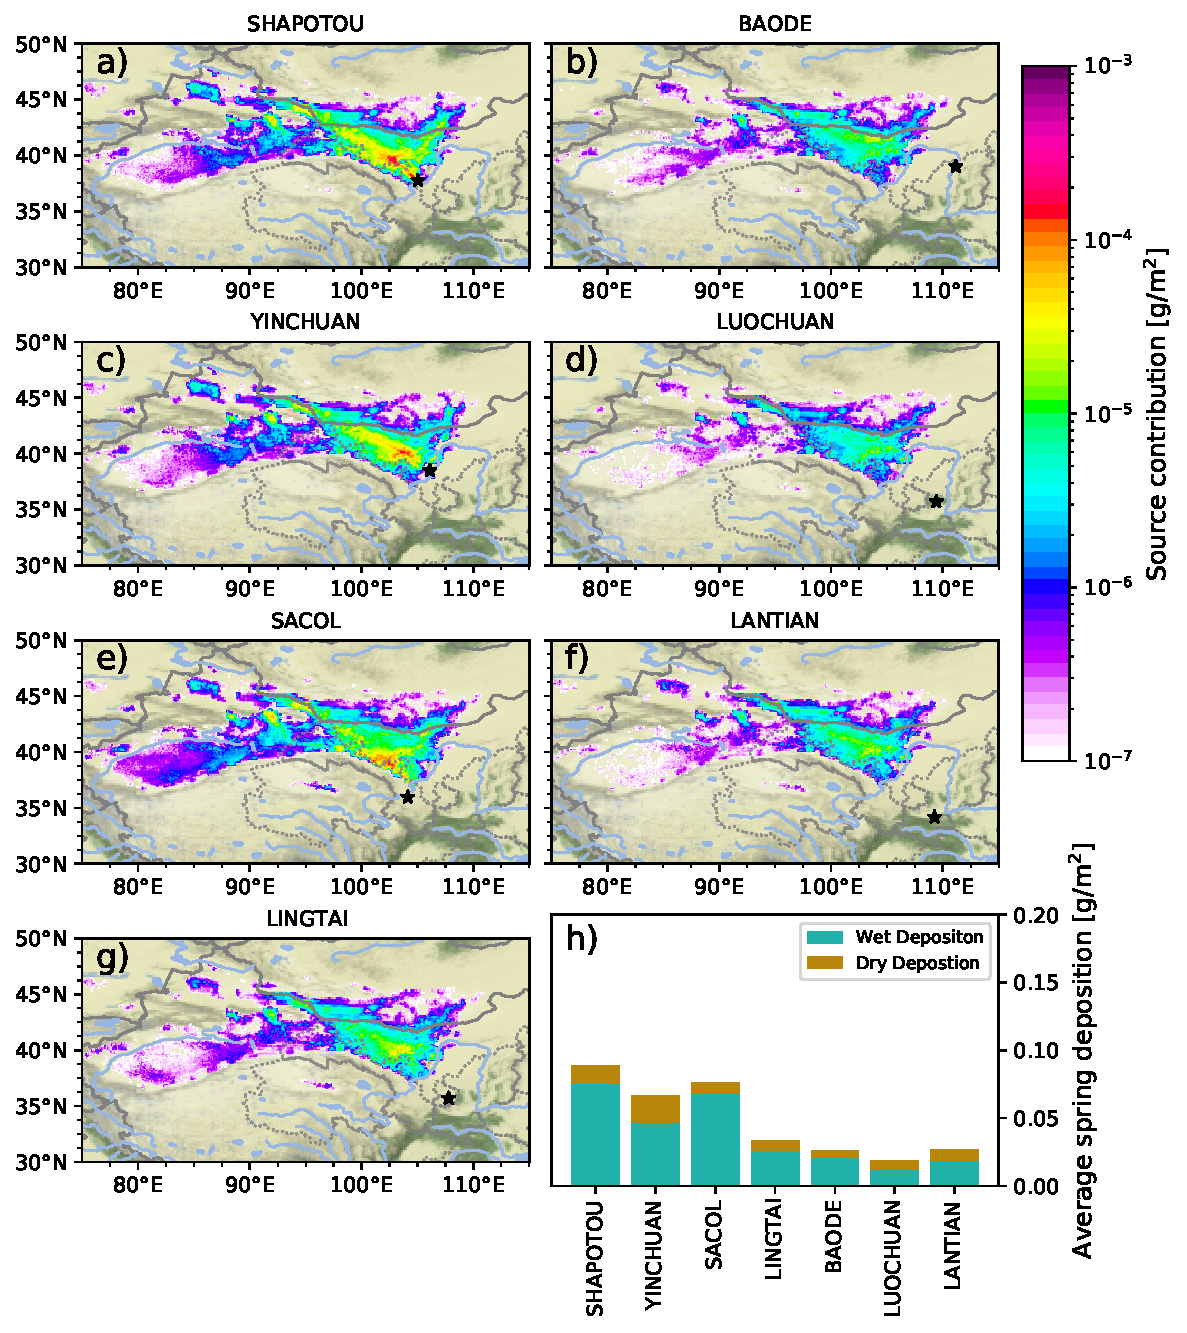
\includegraphics[width=\textwidth]{texfiles/figs/2micron_total_depositon_source_contribution.pdf}
    \caption{Yearly averaged spring source contribution "Fine Clay" dust size bin for the seven sites across the CLP (a-g). Panel h) shows the averaged spring deposition of each site for both wet- and dry deposition}
    \label{fig:source_contrib_2mmu}
\end{figure}

\Cref{fig:source_contrib_2mmu} and \Cref{fig:source_contrib_20mmu} shows the spring averaged source contribution for the coarse and fine particles respectively. The main source contributing to the deposition from all the location is the proximal deserts north west of the CLP.  The western sites, Shapotou, Yinchuan, Sacol and Lingtai have a stronger contribution from Taklamakan compared to the eastern site. \Cref{fig:source_contrib_2mmu}h and \Cref{fig:source_contrib_20mmu}h shows that the primary mode of deposition for all the sites is wet deposition. The wet deposition is even more dominating for the coarse particles. This is consistent with the coarse particle requiring to be transported through the upper troposphere as shown by the average dust loading trajectories as it is more likely that dust particles will be subjected to cloud scavenging.     
 \begin{figure}[htbp]
    \centering
    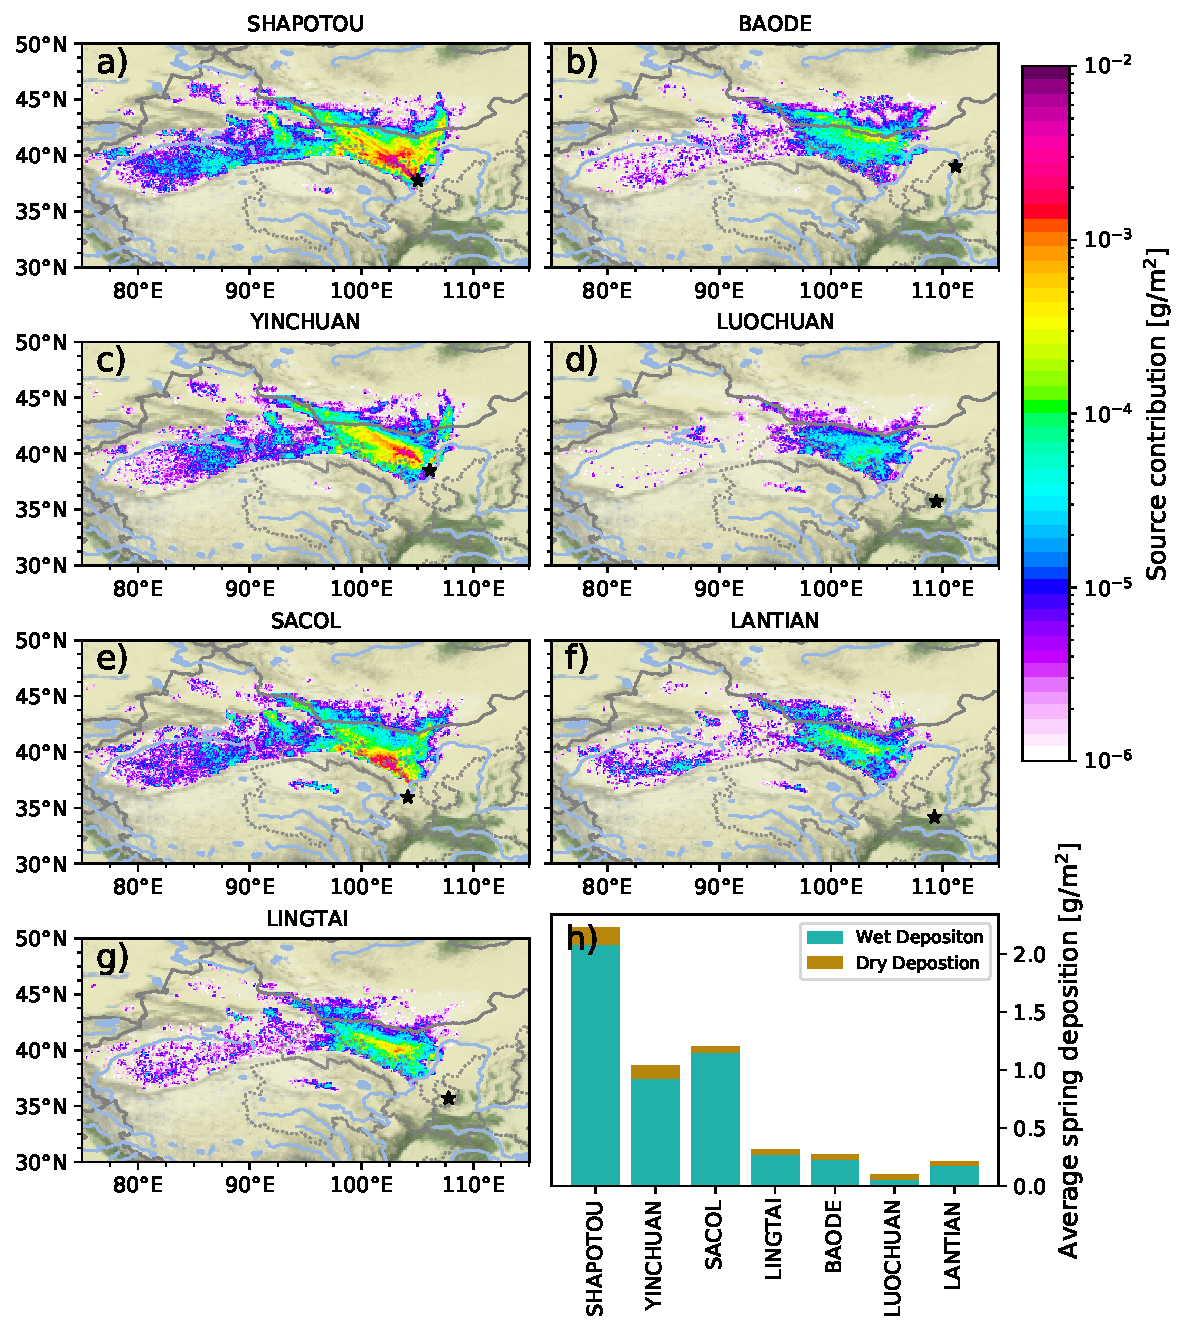
\includegraphics[width=\textwidth]{texfiles/figs/20micron_total_depositon_source_contribution.pdf}
    \caption{Yearly averaged March-May source contribution "Coarse Silt" size bin for the seven sites across the CLP (a-g). Panel h) shows the averaged spring deposition of each site for both wet- and dry deposition}
    \label{fig:source_contrib_20mmu}
\end{figure}

\section{Inter-annual variations in emission, transport and deposition}

\subsection{Inter-annual variation in emissions}
The time series of spring time emissions for the 3 major source regions are shown in \Cref{fig:emission_timeseries}. Over this 20 year period there is no overall trend in the spring time emissions from the East Asian sources. The 3 strongest year overall are identified as 2001, 2010 and 2018. For 2001 and 2010 the North west CLP regions stands for the larges increase in emissions, whereas for 2018 Taklamakan and the Other sources are responsible for the increase in emissions. Years with strong emissions from the North west CLP and generally coincide with enhanced emissions from Mongolia but not always with enhanced emissions from Taklamakan, e.g. 2013.   

\begin{figure}[htbp]
    \centering
    \includegraphics[width=\textwidth]{../figs/Emission_timeseries.pdf}
    \caption{Time series of total spring time dust emissions from 1999-2019. The total emission is partitioned into the contribution from the Taklamakan (Blue), North West CLP (Green) and Mongolia (Orange) }
    \label{fig:emission_timeseries}
\end{figure}
Empirical orthogonal function (EOF) analysis based on yearly de-trended spring emissions was done to identify the main modes of variability in the dust emissions. The significance of each EOF was evaluated based on the rule of thumb outlined by \textcite{north1982sampling}. Which states that if the neighbouring eigenvalue lay within the typically error of the respective eigenvalue $\lambda$, the two EOF might be mixed in their signal and hence not representing true patterns. Following this rule, \Cref{fig:eof_test} shows that the first and second EOF meets this criterion.     

\Cref{fig:emissions_eof}a and b shows the spatial pattern of the two leading EOFs. EOF1 and EOF2 account for 54 \% and 12 \% of the variance in spring time emissions. The leading EOF represent an all over increase in emissions across every source region and as expected the years with a large positive principal component correspond to to strong emissions years. Interestingly the second EOF on show a dipole pattern between emissions in Mongolia and emissions from Taklamakan.    


\begin{figure}[htbp]
    \centering
    \includegraphics[width=\textwidth]{texfiles/figs/Emissions_EOF.pdf}
    \caption{The spatial pattern of the leading EOF (a) and second EOF (b). (c) the time series of the normalized principal component of the first (purple) and second (blue) EOFs.}
    \label{fig:emissions_eof}
\end{figure}



\begin{figure}[htbp]
    \centering
    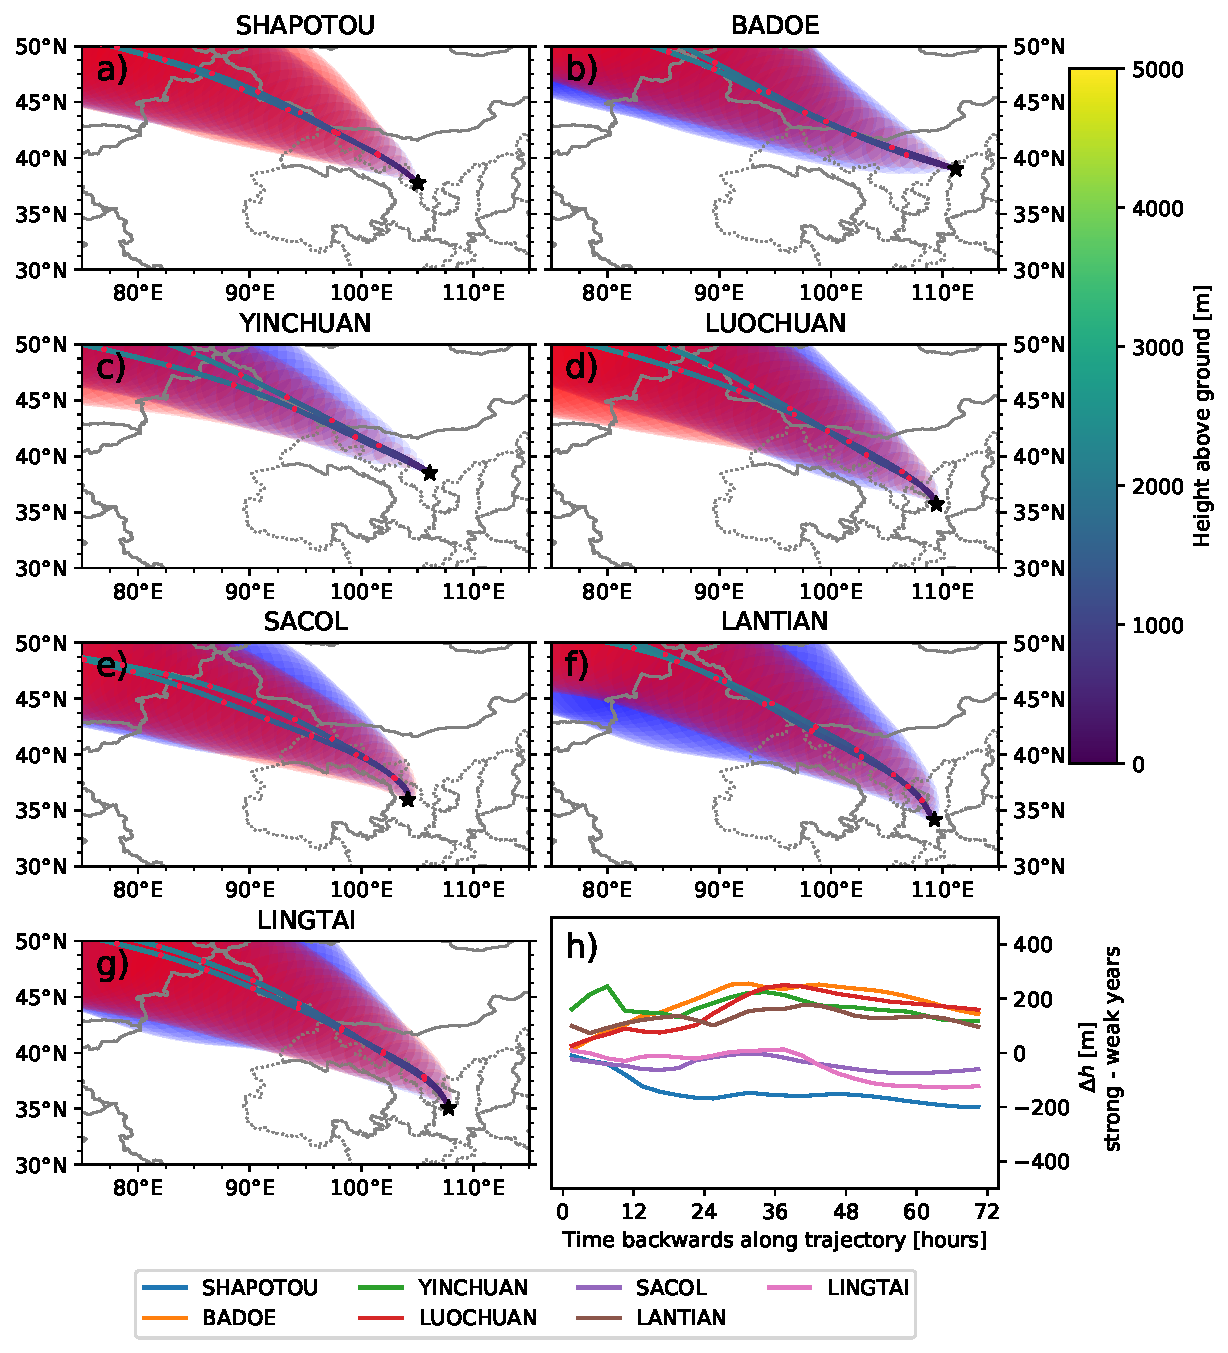
\includegraphics[width=\textwidth]{texfiles/figs/2_micron_drydep_weak_strong_trajecs .pdf}
    \caption{The weighted average of dust loading trajectories for strong and weak deposition years for all locations. The standard deviation for of the trajectories during the weak deposition and strong deposition years are reperesented by blue and red shading respectively.  }
    \label{fig:strong_weak_depo_year_2mmu_trajecs}
\end{figure}
\begin{figure}[htbp]
    \centering
    \includegraphics[scale=0.7]{texfiles/figs/EOF_north_test.pdf}
    \caption{The eigenvalues of the 10 first leading EOFs. The error bars correspond to the typical error of each EOF}
    \label{fig:eof_test}
\end{figure}






\begin{figure}[hptb]
    \centering
    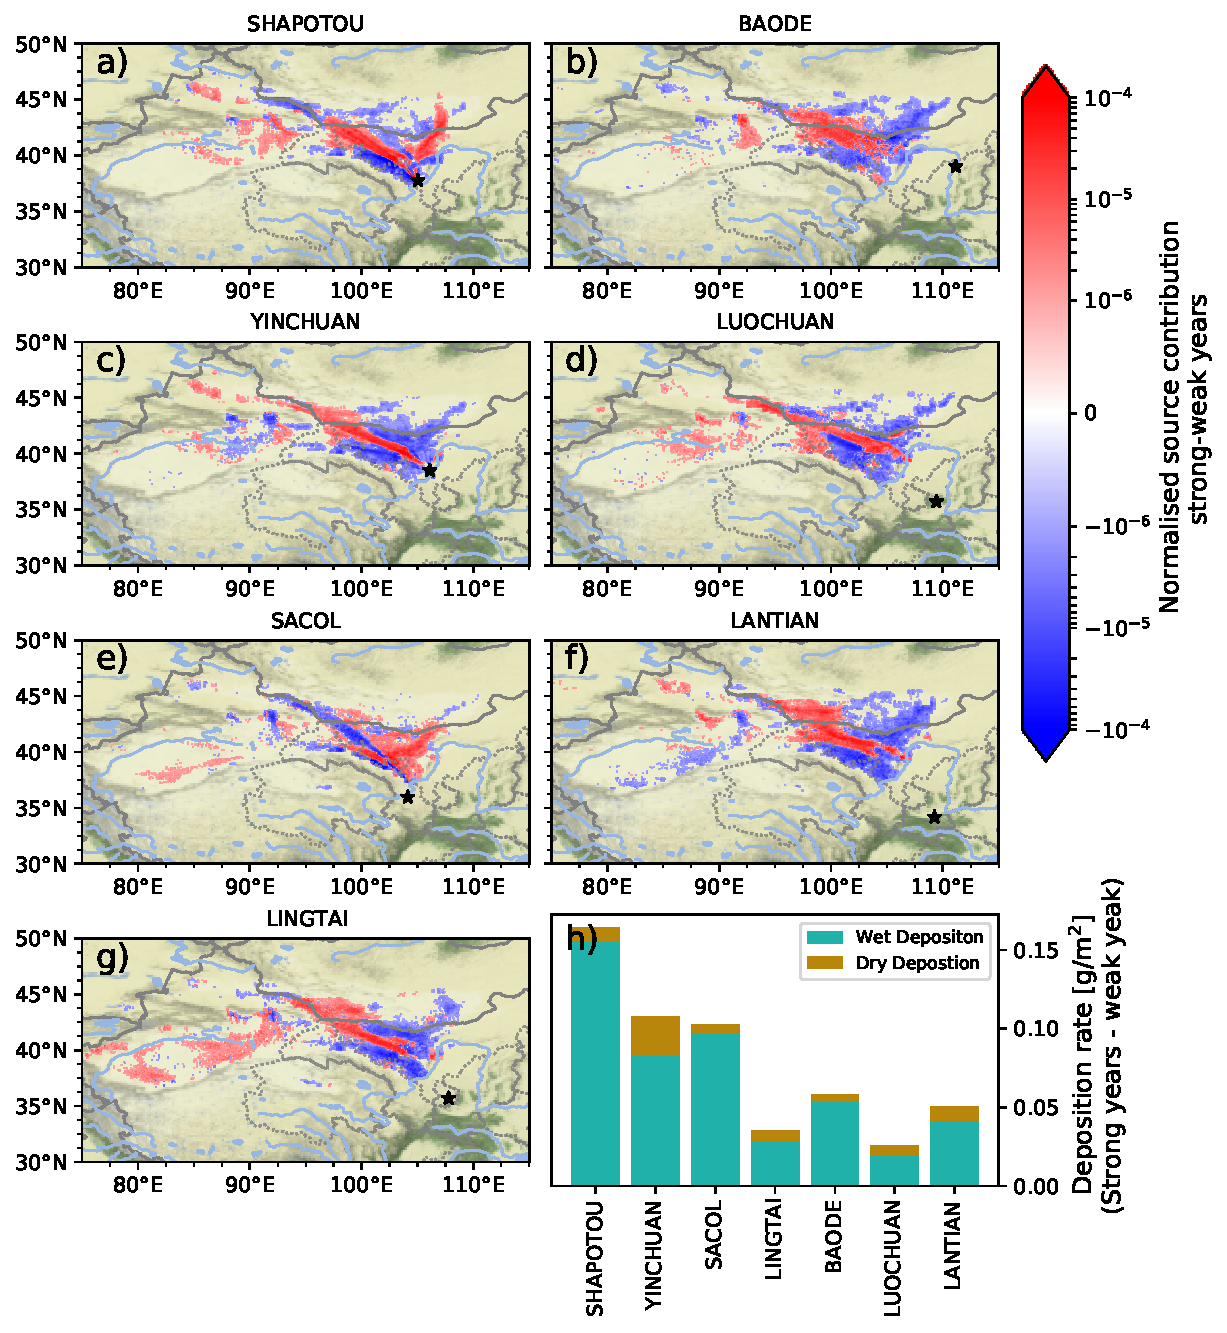
\includegraphics[width=\textwidth]{texfiles/figs/composite_source_contrib_2micron_tot_dep.pdf}
    \caption{Normalised source contribution composite anomalies of "fine clay" particle size bin for all locations, strong - weak deposition years.}
    \label{fig:source_contrib2mmu_anomalies}
\end{figure}

\begin{figure}[hptb]
    \centering
    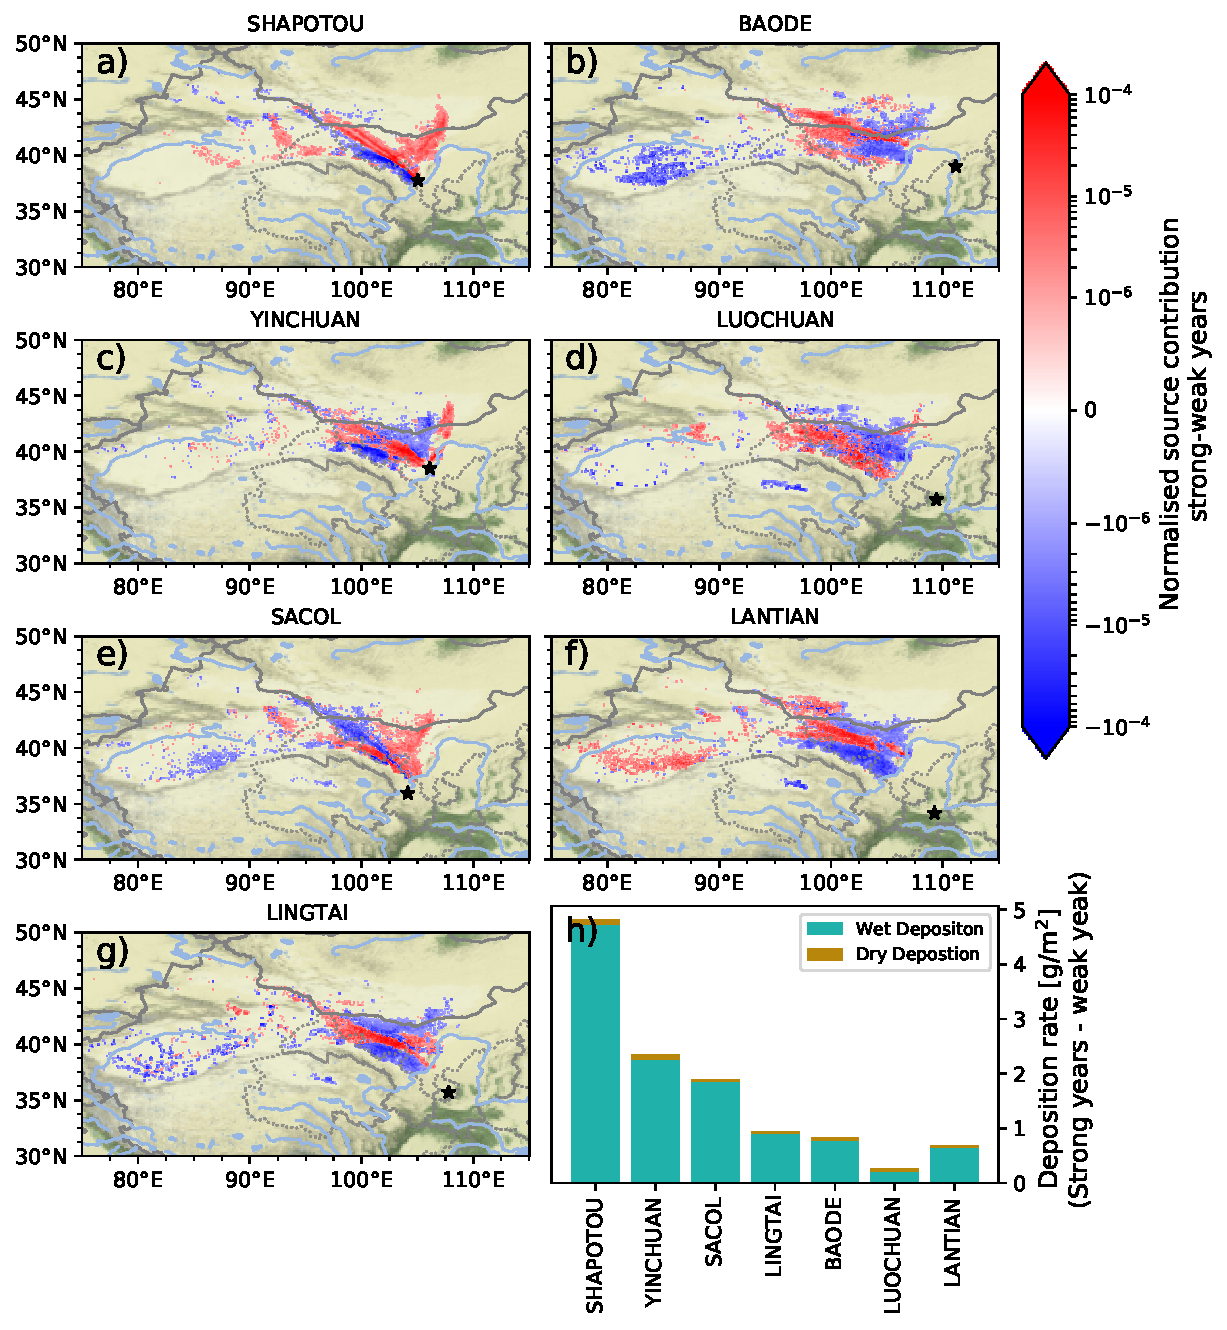
\includegraphics[width=\textwidth]{texfiles/figs/composite_source_contrib_20micron_tot_dep.pdf}
    \caption{Normalised source contribution composite anomalies of "coarse silt" particle size bin for all locations, strong - weak deposition years.}
    \label{fig:source_contrib20mmu_anomalies}
\end{figure}

\begin{figure}[htpb]
    \centering
    \includegraphics[width=\textwidth]{../figs/correlations.pdf}
    \caption{Inter annual correlations between deposition and each site and local and large-scale climate indices. The significant correlations are indicated}
    \label{fig:correlations}
\end{figure}


\begin{figure}
    \centering
    \includegraphics[width=\textwidth]{texfiles/figs/winter_MO_AO_composite.pdf}
    \caption{Circulation composite anomalies of 850hPa winds and mean sea level pressure for strong - weak winter monsoon years and negative - positive winter AO. (a) and (b) is the DJF anomalies and (c) - (d) is MAM anomilies in the following spring}
    \label{fig:mo_ao_composite}
\end{figure}

\begin{figure}
    \centering
    \includegraphics[width=\textwidth]{texfiles/figs/winter_MO_AO_composite_500h.pdf}
    \caption{Circulation composite anomalies of 500hPa winds and geopotential height for strong - weak winter monsoon years and negative - positive winter AO. (a) and (b) is the DJF anomalies and (c) - (d) is MAM anomilies in the following spring}
    \label{fig:mo_ao_composite_500hPa}
\end{figure}

\begin{figure}[hp]
    \centering
    \includegraphics[width=\textwidth]{texfiles/figs/mslp_850hPa_20micron_DJF.pdf}
    \caption{Composite difference anomalies of mean sea level pressure and 850hPa strong minus weak deposition years of the "coarse silt" size bin in winter for all the locations (a-g).  (h) indicates which years are strong years and which years are weak.}
    \label{fig:DJF_850_coarse_composite}
\end{figure}

\begin{figure}[hp]
    \centering
    \includegraphics[width=\columnwidth]{texfiles/figs/mslp_850hPa_2micron_DJF.pdf}
    \caption{Composite difference anomalies of mean sea level pressure and 850hPa strong minus weak deposition years of the "fine clay" size bin in winter for all the locations (a-g). (h) indicates which years are strong years and which years are weak.}
    \label{fig:DJF_850_fine_composite}
\end{figure}

\begin{figure}[hptb]
    \centering
    \includegraphics[width=\columnwidth]{texfiles/figs/20micrion_DJF_ws_geopot_500hPa.pdf}
    \caption{Caption}
    \label{fig:DJF_500hPa_coarse_composite}
\end{figure}

\begin{figure}[hptb]
    \centering
    \includegraphics[width=\columnwidth]{texfiles/figs/2micrion_DJF_ws_geopot_500hPa.pdf}
    \caption{Caption}
    \label{fig:DJF_500hPa_fine_composite}
\end{figure}